
\documentclass{beamer}
\usepackage[latin1]{inputenc}
%\usetheme{Montpellier}
%\usetheme{Boadilla}
%\usecolortheme[RGB={204,51,255}]{structure}
%\usecolortheme[named=purple]{structure}
%\usecolortheme[RGB={62,128,62}]{structure}
\usecolortheme[RGB={62,62,128}]{structure}
%\definecolor{reddish}{rgb}{0.3,0.15,0.3}
%\definecolor{light}{rgb}{0.8,0.6,0.8}
%\definecolor{reddish}{rgb}{.5,0.15,0.15}
\definecolor{reddish}{rgb}{0.5,0.3,0.4}
%\definecolor{light}{rgb}{0.8,0.6,0.8}
\definecolor{reddish}{rgb}{.7,0.25,0.25}
\definecolor{greenish}{rgb}{.25,0.8,0.25}
\definecolor{blueish}{rgb}{.25,0.25,0.7}
\definecolor{purple}{rgb}{.5,0.0,0.5}
\usepackage{graphicx}
\usepackage{pstricks}
\usepackage{epsfig}
\newcommand{\btVFill}{\vskip0pt plus 1filll}

\setbeamertemplate{navigation symbols}{}

\newcommand{\crish}{\color{reddish}}
\newcommand{\cgish}{\color{greenish}}
\newcommand{\cbla}{\color{black}}
\newcommand{\cred}{\color{red}}
\newcommand{\cblu}{\color{blue}}
\newcommand{\cgrish}{\color{green}}

\newcommand{\sm}{\color{reddish}$}
\newcommand{\fm}{$\color{black}{}}

\newcommand{\letter}[1]{\color{blue}\texttt{#1}\color{black}}
\newcommand{\binary}[1]{\color{red}\texttt{#1}\color{black}}

\usepackage{tikz}
\usetikzlibrary{arrows,decorations.markings,positioning}
\usepackage{epstopdf}
\usetikzlibrary{fit}
\usepackage{pgfplots}

\title[The Bayesian Brain lecture 1]{The Bayesian approach: the Bayesian Brain lecture 1}
\author{COMSM0094 Learning Computation and the Brain}
\institute{\texttt{comsm0075.github.io}}
\date{November 2021}

\begin{document}

\maketitle


\begin{frame}{Bayes's rule}
  \crish$$
  P(X|Y)=\frac{P(Y|X)P(X)}{P(Y)}
  $$\cbla
\end{frame}


\begin{frame}{The compulsory xkcd cartoon}
\begin{center}
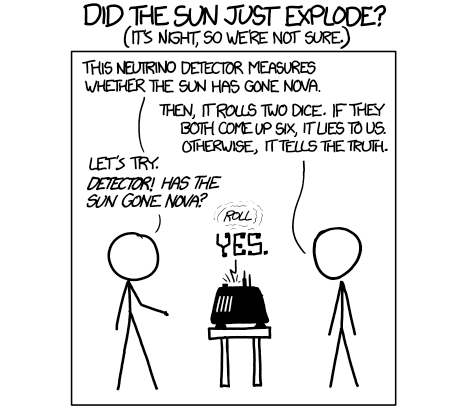
\includegraphics[width=7.5cm]{xkcd1.png}
\end{center}
\vfill
\flushright{\tiny{xkcd.com/1132/}}
\end{frame}


\begin{frame}{The compulsary xkcd cartoon}
\begin{center}
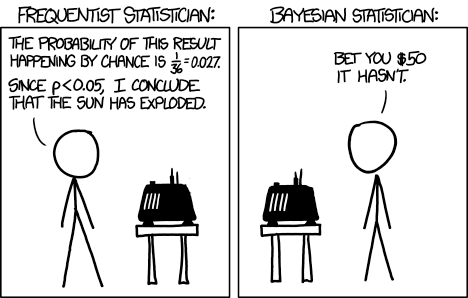
\includegraphics[width=8.5cm]{xkcd2.png}
\end{center}
\vfill
\flushright{\tiny{xkcd.com/1132/}}
\end{frame}

\begin{frame}{Recall Bayes's rule}
  \crish$$
  P(X|Y)=\frac{P(Y|X)P(X)}{P(Y)}
  $$\cbla
\end{frame}

\begin{frame}{xkcd maths}
  \crish$D$\cbla{} is the state of the detector with
  \crish$D=\cred{}w$\cbla{} corresponding to a \cred{}warning\cbla{}.
\begin{center}

\includegraphics[width=1.5cm]{xkcd_detector.png}
\end{center}
\end{frame}


\begin{frame}{xkcd maths}
  \crish$S$\cbla{} is the state of the \color{orange}sun\cbla{} with
  \crish$S=\cred{}n$\cbla{}  corresponding to a \cred{}nova\cbla{} and \crish$S=\cblu{}f$\cbla{} to it staying fine. 
\begin{center}
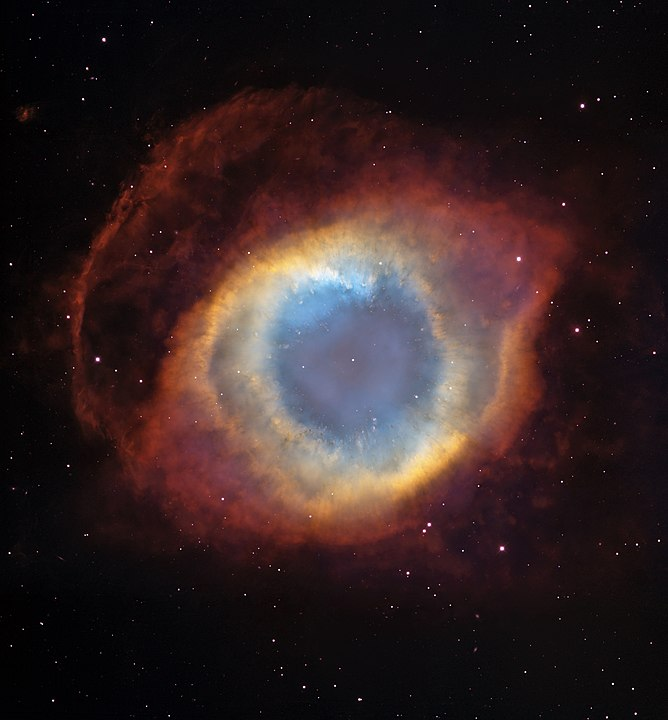
\includegraphics[width=5cm]{nebula.jpg}
\end{center}
\vfill
\flushright{\tiny{Picture of the Helix nebula from Wikipedia}}
\end{frame}


\begin{frame}{xkcd math}
    The cartoon tells us that
  \crish$$
  P(D=w|S=f)=\frac{1}{36}
  $$\cbla{}
  \flushleft{and since this is close to zero, the silly frequentist assumes the sun
    has exploded.}
  \end{frame}


\begin{frame}{xkcd math}
  The cartoon tells us that
  \crish$$
  P(D=w|S=n)=\frac{35}{36}
  $$\cbla{}
\flushleft{Let's assume the probability the sun has exploded is one
in a million; it is actually much less than that, so}
\crish$$
P(S=n)=10^{-6}
$$\cbla{}
We want to know
\crish$$
P(S=f|D=w)=\frac{P(D=w|S=f)P(S=f)}{P(D=w)}
$$\cbla{}
\end{frame}


\begin{frame}{xkcd math}
\crish$$
P(S=f|D=w)=\frac{P(D=w|S=f)P(S=f)}{P(D=w)}
$$\cbla{}
Numerator is easy:
\crish$$
P(D=w|S=f)P(S=f)=\frac{1}{36}(1-10^{-6})
$$\cbla{}
The denominator requires marginalizing:
\crish$$
P(D=w)=P(D=w,S=n)+P(D=w,S=f)
$$\cbla{}
\vskip 1cm
Doing what's required gives
\crish$$
P(S=f|D=w)\approx 0.999965
$$\cbla{}
\end{frame}

\begin{frame}{The Bayesian brain}
  \begin{quote}The point of this section is that the brain appears to perform Bayesian calculation over multiple pieces of evidence incorporating recent observations and established models of the world.
  \end{quote}
\end{frame}

\begin{frame}{What does probability model?}
  \begin{quote}
    The laws of probability are mathematics - the mathematics don't determine what probabilities model.
    \end{quote}
\end{frame}

\begin{frame}{Frequentists versus Bayesians}
  \begin{center}
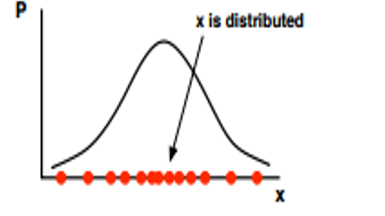
\includegraphics[width=4.125cm]{fig_freq.png}
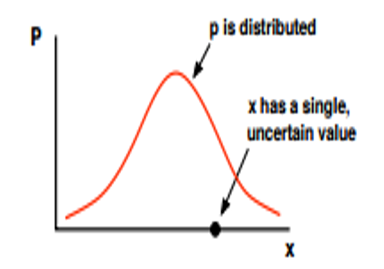
\includegraphics[width=3.75cm]{fig_bayes.png}
\end{center}
  \vfill
\flushright{\tiny{Picture from Rosalyn Moran}}  
\end{frame}

\begin{frame}{Guess the missing letter}
  \begin{tabular}{lc}
    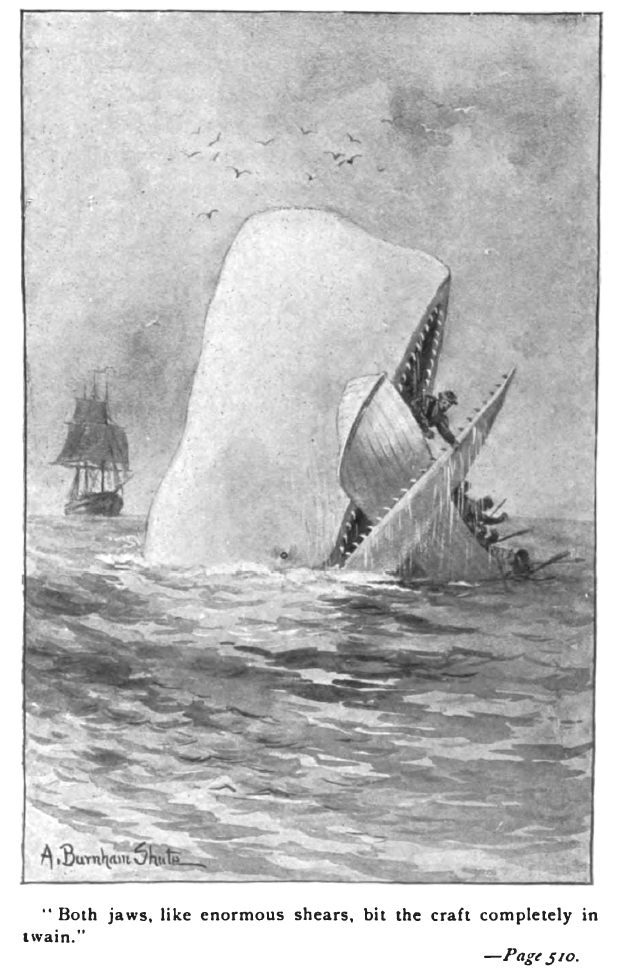
\includegraphics[width=4cm]{Moby_Dick.jpg}&\cred{}CALL ME ISHMAE*\cbla{}
  \end{tabular}
  \end{frame}


\begin{frame}{Guess the missing letter - letter frequencies}
  \begin{center}
    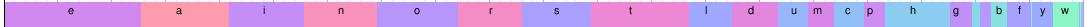
\includegraphics[width=11cm]{freq.png}
  \vskip 1cm
    \cred{}CALL ME ISHMAE\cblu{}*\cbla{}
  \end{center}
  with for example \crish$p(E)=0.13$\cbla{}, \crish$p(L)=0.04$\cbla{} and \crish$p(Q)=0.001$\cbla{}. 
  \vfill
  \flushright{\tiny{Letter frequency table from Wikipedia}}  
  \end{frame}


\begin{frame}{Guess the missing letter - 2-gram letter frequencies}
  Look at two letter pairs, \textsl{ER} and \textsl{EL} and so on, and
  work out conditional probabilities like \crish$$ p(\mbox{second
    letter is L}|\mbox{first letter is E})
  $$\cbla{}
  \begin{center}
    \cred{}CALL ME ISHMA\cblu{}E*\cbla{}
  \end{center}
  with for example \crish$p(R)=0.14$\cbla{}, \crish$p(L)=0.04$\cbla{} and \crish$p(Q)=0.003$\cbla{}. 
  \end{frame}


\begin{frame}{Guess the missing letter - 3-gram letter frequencies}


    \begin{center}
    \cred{}CALL ME ISHM\cblu{}AE*\cbla{}
  \end{center}
  with for example \crish$p(R)=0.1$\cbla{}, \crish$p(L)=0.4$\cbla{} and \crish$p(P)=0.001$\cbla{}. 
  \end{frame}


\begin{frame}{Guess the missing letter}
  \begin{tabular}{lc}
    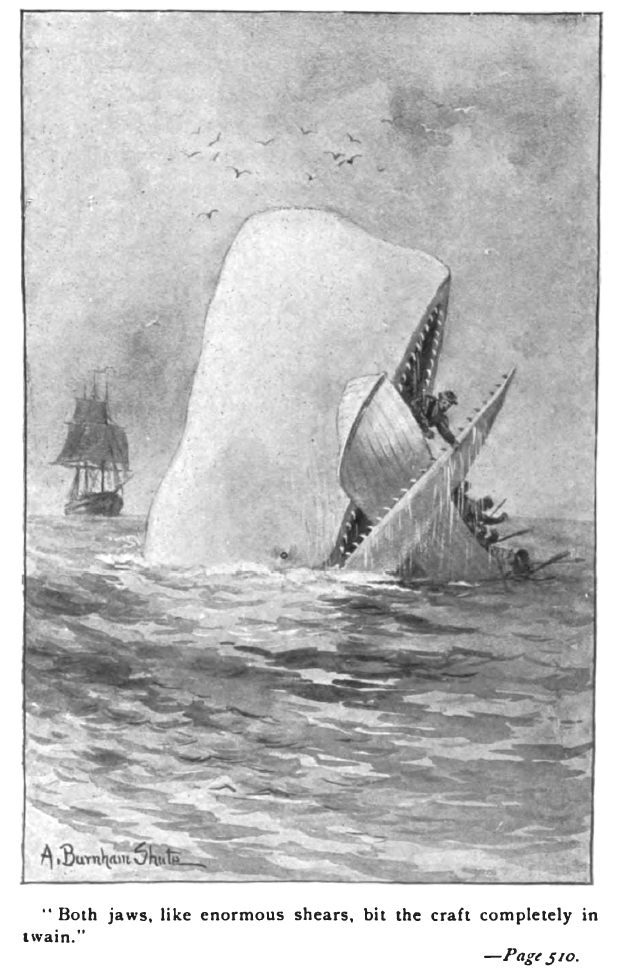
\includegraphics[width=4cm]{Moby_Dick.jpg}&\cred{}CALL ME ISHMAEL\cbla{}
  \end{tabular}
  \end{frame}

\begin{frame}{The Bayesian brain}

  \begin{quote}
    The problem the brain faces is a Bayesian one, the brain
gathers evidence about the world through the senses, these are
unreliable and limited but the brain has to infer the state of the
world from the information they provided.
  \end{quote}
\end{frame}

\begin{frame}{Bayes's rule}
In a Bayesian interpretation Bayes's rule 
\crish$$
P(W|E)=\frac{P(E|W)P(W)}{P(E)}
$$\cbla{}
\flushleft{allows us to update our view of the world \crish$W$\cbla{} based on evidence \crish$E$\cbla. The rule is described as an update rule:}
\crish$$
\mbox{posterior}=\frac{\mbox{likelihood}\times \mbox{prior}}{\mbox{evidence}}
$$\cbla{}
\end{frame}

\begin{frame}{Bayes's rule}
\crish$$
\mbox{posterior}=\frac{\mbox{likelihood}\times \mbox{prior}}{\mbox{evidence}}
$$\cbla{}
\vskip 1cm
The \textbf{prior}, is our belief about the world before our
observation, the \textbf{likelihood} is the probability of the
evidence given the state of the world \crish$P(E|W)$\cbla, the
\textbf{evidence} is the probability of the evidence
\crish$P(W)$\cbla{} and the \textbf{posterior}, \crish$P(W|E)$\cbla, is our new
belief about the world given the evidence we have observed.
\end{frame}
  

\end{document}

